\chapter{实验数据与处理}

\section{内外润滑剂组合对 CPVC 性能的影响}

\subsection{配方设计}
由上一组实验我们得到 PEW-0380 外润滑剂具有最好的综合润滑性能,因此在本组实验中我们选用 PEW-0380/G-60 润滑剂组合作为对照组,并且使用 A 蜡和 OP 蜡两种外润滑剂以及 OA2 蜡和 E 蜡两种内润滑剂两两组合配方,共 5 组配方做为实验组进行热稳定性和力学性能的测试。探究内外润滑剂对于 CPVC 热稳定性和加工性能的协同影响。具体配方如表 \ref{tab2Pre} 所示。

\begin{table}[!htb]
    \caption{CPVC 内外润滑剂组合配方设计表}
    \label{tab2Pre}
    \begin{center}
    \footnotesize{
        \begin{tabular}{cccccccccccc}
            \Xhline{1pt}
            \multirow{2}{*}{\makecell[c]{组别}} & \multirow{2}{*}{\makecell[c]{CPVC}} & \multirow{2}{*}{\makecell[c]{抗冲击\\改性剂}} & \multirow{2}{*}{\makecell[c]{有机锡}} & \multicolumn{3}{c}{外润滑剂} & \multicolumn{3}{c}{内润滑剂} & \multirow{2}{*}{\makecell[c]{加工\\助剂}} & \multirow{2}{*}{\makecell[c]{钛白粉}}   \\
            \cline{5-10}
            &&&& \makecell[c]{PEW-0380} & A 蜡 &  OP 蜡 & G-60 & OA2 蜡 & E 蜡	\\ 
            \Xhline{0.5pt}
            $S_1$ & 100 & 8 & 2 & 1.3 & & & 1.2 & & & 3 & 2	\\
            $S_2$ & 100 & 8 & 2 & & 1.3 & & & 1.2 & & 3 & 2	\\
            $S_3$ & 100 & 8 & 2 & & 1.3 & & & & 1.2 & 3 & 2	\\
            $S_4$ & 100 & 8 & 2 & & & 1.3 & & 1.2 & & 3 & 2	\\
            $S_5$ & 100 & 8 & 2 & & & 1.3 & & & 1.2 & 3 & 2	\\
            \Xhline{1pt}
        \end{tabular}
    }
    \end{center}
\end{table}

\subsection{玻璃化转变温度}

根据 $S_1 \sim S_5$ 五组配方的 损耗因子-时间 数据制得图 \ref{fig2Tg},取损耗因子的峰值温度作为试样的玻璃化转变温度。

\begin{figure}[!htb]
    \begin{center}
        % GNUPLOT: LaTeX picture with Postscript
\begingroup
  \makeatletter
  \providecommand\color[2][]{%
    \GenericError{(gnuplot) \space\space\space\@spaces}{%
      Package color not loaded in conjunction with
      terminal option `colourtext'%
    }{See the gnuplot documentation for explanation.%
    }{Either use 'blacktext' in gnuplot or load the package
      color.sty in LaTeX.}%
    \renewcommand\color[2][]{}%
  }%
  \providecommand\includegraphics[2][]{%
    \GenericError{(gnuplot) \space\space\space\@spaces}{%
      Package graphicx or graphics not loaded%
    }{See the gnuplot documentation for explanation.%
    }{The gnuplot epslatex terminal needs graphicx.sty or graphics.sty.}%
    \renewcommand\includegraphics[2][]{}%
  }%
  \providecommand\rotatebox[2]{#2}%
  \@ifundefined{ifGPcolor}{%
    \newif\ifGPcolor
    \GPcolorfalse
  }{}%
  \@ifundefined{ifGPblacktext}{%
    \newif\ifGPblacktext
    \GPblacktexttrue
  }{}%
  % define a \g@addto@macro without @ in the name:
  \let\gplgaddtomacro\g@addto@macro
  % define empty templates for all commands taking text:
  \gdef\gplbacktext{}%
  \gdef\gplfronttext{}%
  \makeatother
  \ifGPblacktext
    % no textcolor at all
    \def\colorrgb#1{}%
    \def\colorgray#1{}%
  \else
    % gray or color?
    \ifGPcolor
      \def\colorrgb#1{\color[rgb]{#1}}%
      \def\colorgray#1{\color[gray]{#1}}%
      \expandafter\def\csname LTw\endcsname{\color{white}}%
      \expandafter\def\csname LTb\endcsname{\color{black}}%
      \expandafter\def\csname LTa\endcsname{\color{black}}%
      \expandafter\def\csname LT0\endcsname{\color[rgb]{1,0,0}}%
      \expandafter\def\csname LT1\endcsname{\color[rgb]{0,1,0}}%
      \expandafter\def\csname LT2\endcsname{\color[rgb]{0,0,1}}%
      \expandafter\def\csname LT3\endcsname{\color[rgb]{1,0,1}}%
      \expandafter\def\csname LT4\endcsname{\color[rgb]{0,1,1}}%
      \expandafter\def\csname LT5\endcsname{\color[rgb]{1,1,0}}%
      \expandafter\def\csname LT6\endcsname{\color[rgb]{0,0,0}}%
      \expandafter\def\csname LT7\endcsname{\color[rgb]{1,0.3,0}}%
      \expandafter\def\csname LT8\endcsname{\color[rgb]{0.5,0.5,0.5}}%
    \else
      % gray
      \def\colorrgb#1{\color{black}}%
      \def\colorgray#1{\color[gray]{#1}}%
      \expandafter\def\csname LTw\endcsname{\color{white}}%
      \expandafter\def\csname LTb\endcsname{\color{black}}%
      \expandafter\def\csname LTa\endcsname{\color{black}}%
      \expandafter\def\csname LT0\endcsname{\color{black}}%
      \expandafter\def\csname LT1\endcsname{\color{black}}%
      \expandafter\def\csname LT2\endcsname{\color{black}}%
      \expandafter\def\csname LT3\endcsname{\color{black}}%
      \expandafter\def\csname LT4\endcsname{\color{black}}%
      \expandafter\def\csname LT5\endcsname{\color{black}}%
      \expandafter\def\csname LT6\endcsname{\color{black}}%
      \expandafter\def\csname LT7\endcsname{\color{black}}%
      \expandafter\def\csname LT8\endcsname{\color{black}}%
    \fi
  \fi
    \setlength{\unitlength}{0.0500bp}%
    \ifx\gptboxheight\undefined%
      \newlength{\gptboxheight}%
      \newlength{\gptboxwidth}%
      \newsavebox{\gptboxtext}%
    \fi%
    \setlength{\fboxrule}{0.5pt}%
    \setlength{\fboxsep}{1pt}%
\begin{picture}(7200.00,5040.00)%
    \gplgaddtomacro\gplbacktext{%
      \csname LTb\endcsname%
      \put(814,704){\makebox(0,0)[r]{\strut{}$0$}}%
      \put(814,1518){\makebox(0,0)[r]{\strut{}$0.2$}}%
      \put(814,2332){\makebox(0,0)[r]{\strut{}$0.4$}}%
      \put(814,3147){\makebox(0,0)[r]{\strut{}$0.6$}}%
      \put(814,3961){\makebox(0,0)[r]{\strut{}$0.8$}}%
      \put(814,4775){\makebox(0,0)[r]{\strut{}$1$}}%
      \put(946,484){\makebox(0,0){\strut{}$40$}}%
      \put(1678,484){\makebox(0,0){\strut{}$60$}}%
      \put(2410,484){\makebox(0,0){\strut{}$80$}}%
      \put(3142,484){\makebox(0,0){\strut{}$100$}}%
      \put(3875,484){\makebox(0,0){\strut{}$120$}}%
      \put(4607,484){\makebox(0,0){\strut{}$140$}}%
      \put(5339,484){\makebox(0,0){\strut{}$160$}}%
      \put(6071,484){\makebox(0,0){\strut{}$180$}}%
      \put(6803,484){\makebox(0,0){\strut{}$200$}}%
      \put(2951,4368){\makebox(0,0)[l]{\strut{}144.67\cd}}%
      \put(3083,3554){\makebox(0,0)[l]{\strut{}145.8\cd}}%
      \put(4577,4478){\makebox(0,0)[l]{\strut{}148.06\cd}}%
      \put(5705,3961){\makebox(0,0)[l]{\strut{}150.89\cd}}%
      \put(5705,4368){\makebox(0,0)[l]{\strut{}155.42\cd}}%
    }%
    \gplgaddtomacro\gplfronttext{%
      \csname LTb\endcsname%
      \put(176,2739){\rotatebox{-270}{\makebox(0,0){\strut{}损耗因子}}}%
      \put(3874,154){\makebox(0,0){\strut{}温度/\cd}}%
      \csname LTb\endcsname%
      \put(2794,3179){\makebox(0,0)[r]{\strut{}PEW-0380/G-60}}%
      \csname LTb\endcsname%
      \put(2794,2959){\makebox(0,0)[r]{\strut{}A/OA2}}%
      \csname LTb\endcsname%
      \put(2794,2739){\makebox(0,0)[r]{\strut{}A/E}}%
      \csname LTb\endcsname%
      \put(2794,2519){\makebox(0,0)[r]{\strut{}OP/OA2}}%
      \csname LTb\endcsname%
      \put(2794,2299){\makebox(0,0)[r]{\strut{}OP/E}}%
    }%
    \gplbacktext
    \put(0,0){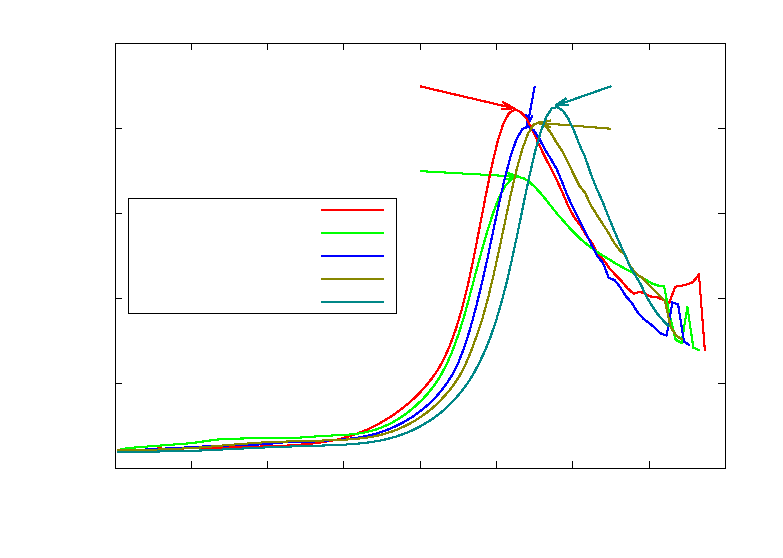
\includegraphics{src/origin/2/tg}}%
    \gplfronttext
  \end{picture}%
\endgroup

    \end{center}
    \caption{外润滑剂玻璃化转变温度}
    \label{fig2Tg}
\end{figure}

\section{热稳定体系测试}

\subsection{动态热稳定性}


\subsection{玻璃化转变温度}

